\chapter{Fundamentação Teórica}
\label{sec:revisao}

Este tópico apresenta conceitos fundamentais sobre Linha de Produto de Software, Experimento e \textit{Quasi}-Experimento em Engenharia de Software, Qualidade de Experimentos e \textit{Quasi}-Experimento em Engenharia de Software, Ontologia e Sistemas de Recomendação tradicional e voltado para Engenharia de Software.

\section{Linha de Produto de Software}
\label{sec:lin_prod_software}

Uma Linha de Produto de Software (LPS) é um conjunto de produtos que endereçam a um determinado segmento de mercado ou missão particular \cite{northrop2007framework}. Esse conjunto de produtos também é denominado família de produtos, no qual os membros desta família são produtos específicos gerados a partir da reutilização de uma infraestrutura comum, denominada núcleo de artefatos (\textit{Core assets}). 

O núcleo de artefatos é composto por um conjunto de características comuns chamadas de similaridades, e características variáveis chamadas de variabilidades \cite{van2007product}. Este núcleo forma a base da LPS que determina a Arquitetura de uma LPS, que são eles, componentes reusáveis, modelos de domínios, requisitos da LPS, planos de testes e modelos de características de variabilidades.

O modelo de características contém todas as características de uma LPS e os seus inter-relacionamentos. De acordo com \citeauthor{apel2013analytic}, "uma característica é um comportamento característico ou visível ao usuário final de um sistema de software". Uma característica pode ser obrigatória, opcional ou alternativa. O modelo de características representa as variabilidades e as variantes de uma LPS \cite{apel2013analytic}.

\begin{itemize}
	\item Variabilidades são descritas por: Ponto de variação que permite a resolução de variabilidades em artefatos genéricos de uma LPS, e; 
	\item Variante é representa pelos: os possessíveis elementos que podem ser escolhidos para resolver um ponto de variação.
\end{itemize}

Restrições entre variantes, estabelecem os relacionamentos entre uma ou mais variantes, com o objetivo de resolver seus respectivos pontos de variação ou variabilidade em um dado tempo de resolução \cite{halmans2003communicating}.

O \textit{MobileMedia} é um exemplo didático de LPS, o produto final é um software que gerencia as mídias de um aparelho celular. O núcleo de artefatos deve conter algumas das seguintes características, opções de criar, visualizar, remover e editar a legenda da imagem. As características variantes opcionais podem ser, a capturar uma nova imagem, ordenar e favoritar imagens. As características variantes alternativas podem ser os diversos tamanhos de tela. O produto final deve possuir ao menos uma variante alternativa.

\begin{figure}[htb]
	\centering					
	{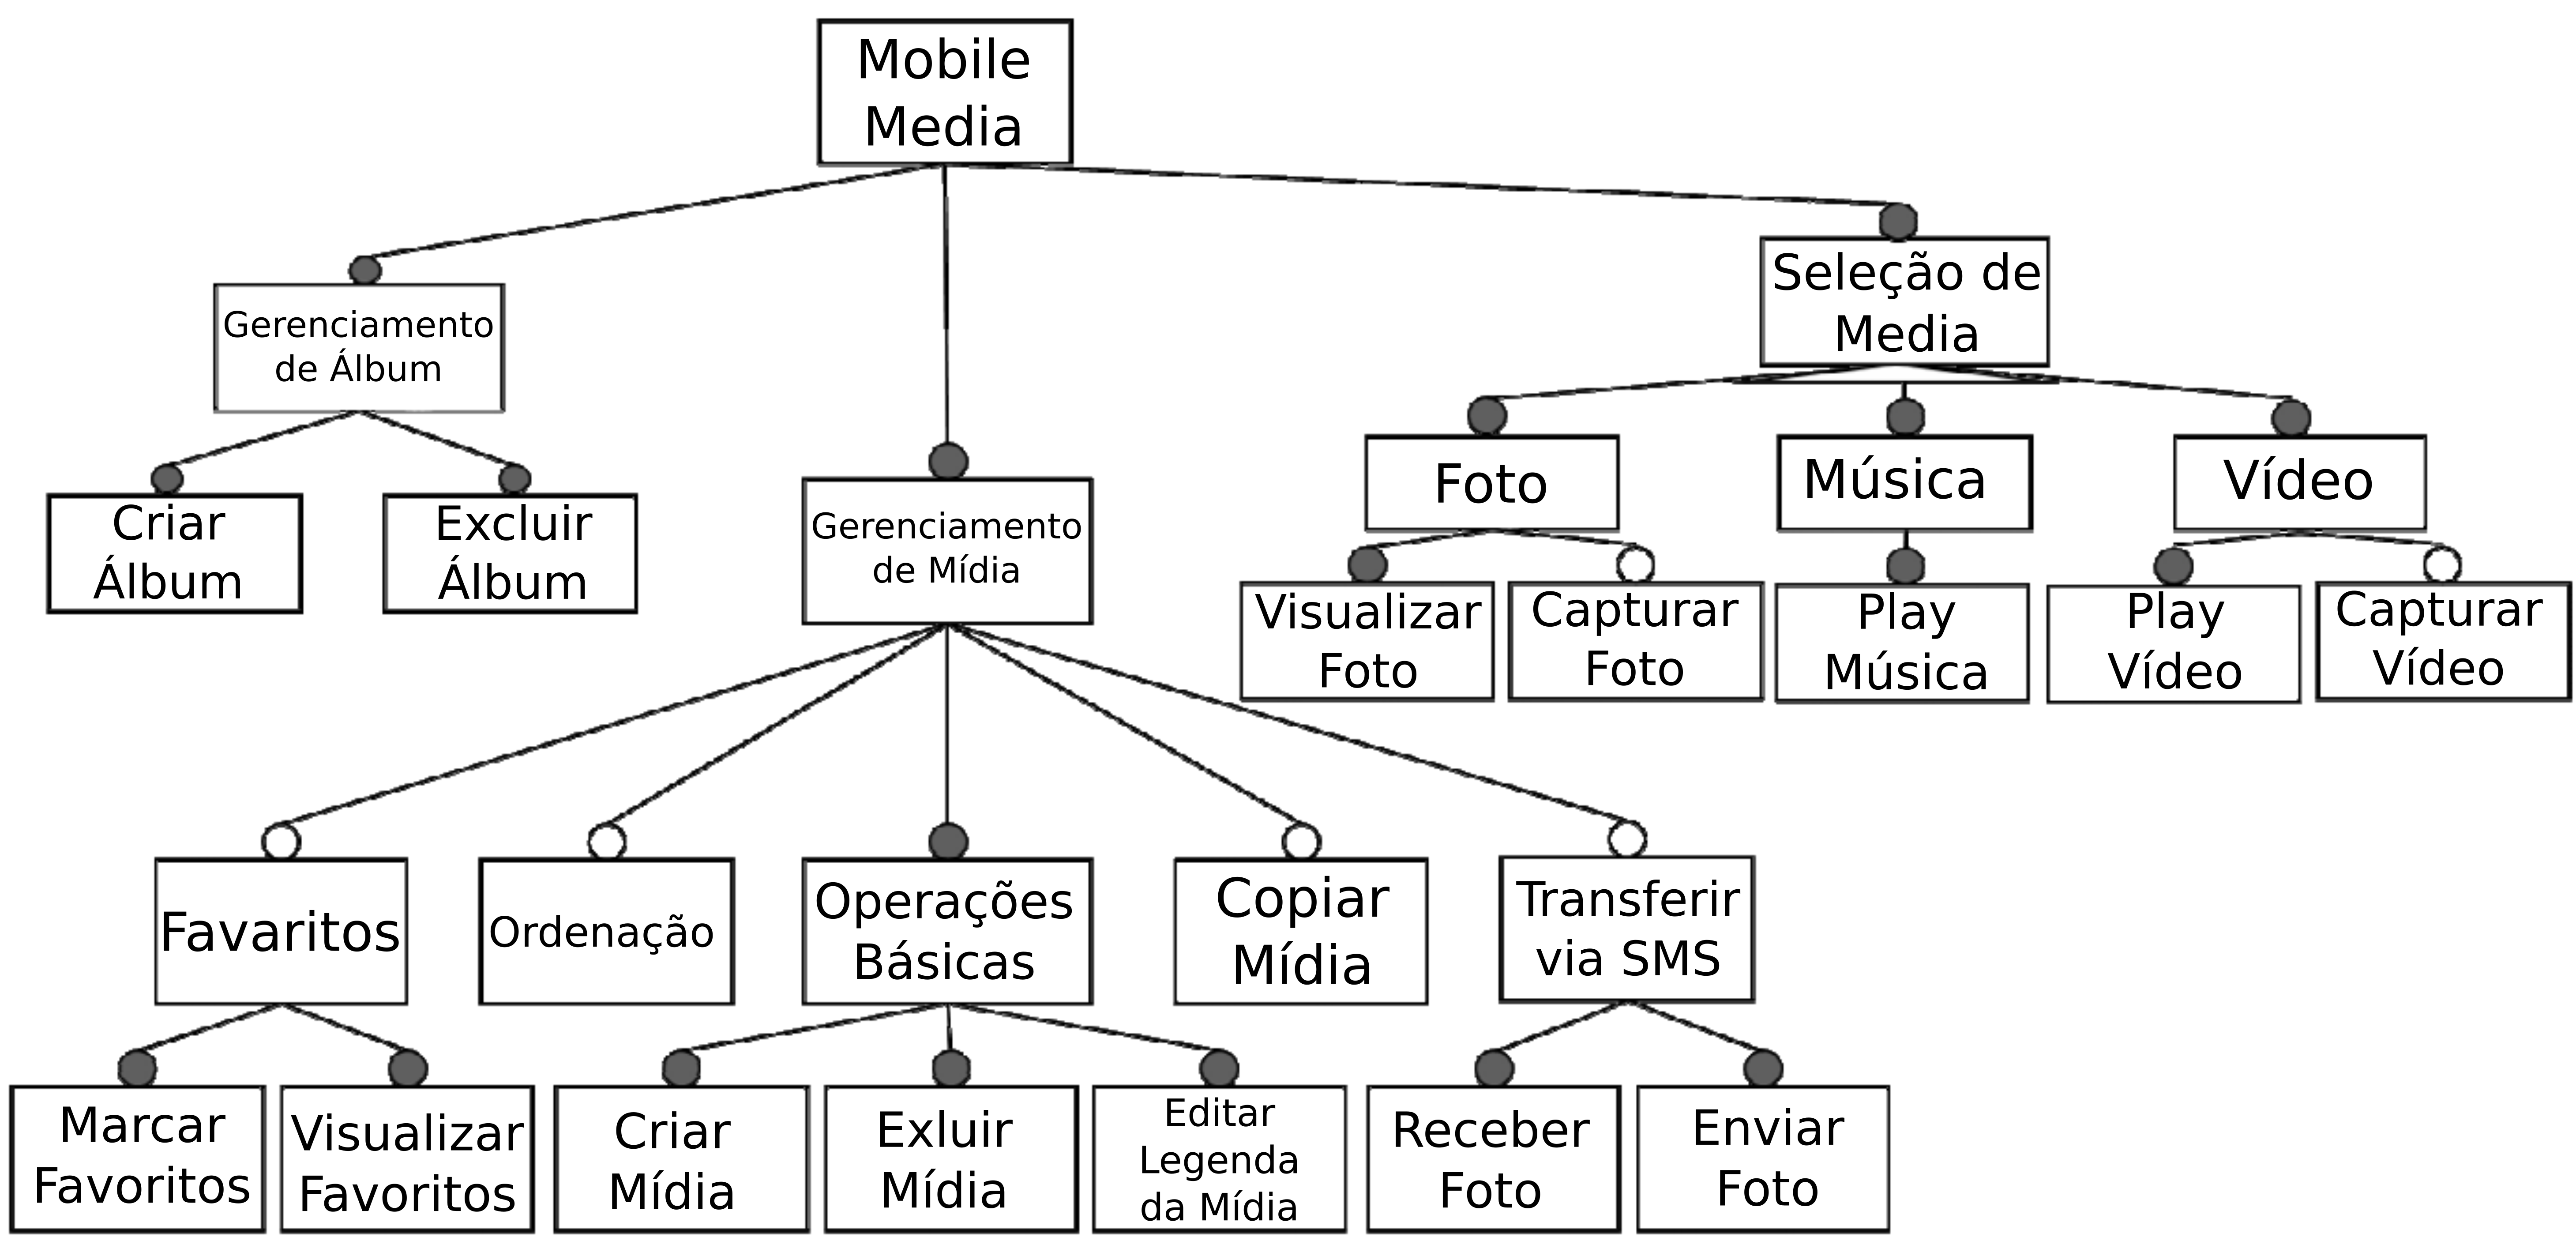
\includegraphics[scale=.33]{exemplo_lps_pt.png}}
	
	\caption{Um modelo de Características. Traduzido de \citet{sommerville2011software} }
	\label{fig:exemplo-lps}
\end{figure}

A \ref{fig:exemplo-lps} apresenta um grafo com o Modelo de Características da LPS \textit{MobileMedia}. As arestas com círculos preenchido representa as características pertencentes ao \textit{core asset}. As arestas com círculos vazios representa características opcionais. As arestas ligadas por um triangulo, como as que saem do vértice Seleção de Mídia, representam características alternativas, por exemplo, uma instância desta LPS deve possuir ao menos um tipo de seleção de mídia, seja ele, por Foto, Música ou Vídeo. 

Uma instancia deste exemplo teria as seguintes características no seu produto de software final:
\begin{itemize}
	\item Gerenciamento de Álbum; 
	\subitem Criar Álbum;
	\subitem Excluir Álbum;
	\item Gerenciamento de Mídia;
	\begin{itemize}
		\item Operações Básicas
		\subitem Criar Mídia
		\subitem Excluir Mídia
		\subitem Editar Legenda Mídia			
		\item Favoritos;
		\subitem Marcar Favoritos
		\subitem Visualizar Favoritos			
	\end{itemize}
	\item Seleção de Mídia;
	\subitem Foto
	\subitem Visualizar Foto
	\subitem Capturar Foto			
\end{itemize}

\citeauthor*{pohl2005software} desenvolveram o \textit{framework} para engenharia de LPS. O objetivo deste de \textit{framework} é incorporar os conceitos centrais da engenharia de linha de produto tradicional, proporcionando a reutilização de artefatos e a customização em massa por meio de variabilidades. O \textit{framework} está dividido em dois processos, o de Engenharia de Domínio e o de Engenharia de Aplicação, conforme apresentado na \ref{fig:framework-lps}.

\begin{itemize}
	\item \textbf{Engenharia de Domínio:} processo em que as similaridades e as variabilidades das LPSs são identificadas e realizadas. No qual, é composto de cinco subprocessos principais, sendo eles: Gerenciamento de Produto, Engenharia de Requisitos do Domínio, Projeto do Domínio, Realização do Domínio e Teste de Domínio;

	\item \textbf{Engenharia de Aplicação:} processo em que as aplicações de uma LPS são construídas por meio da reutilização de artefatos de domínio, explorando as variabilidades de uma linha de produto. No qual, é composto pelos subprocessos: Engenharia de Requisitos da Aplicação, Projeto da Aplicação, Realização da Aplicação e Teste da Aplicação.
\end{itemize}

\begin{figure}[htb]
	\centering					
	{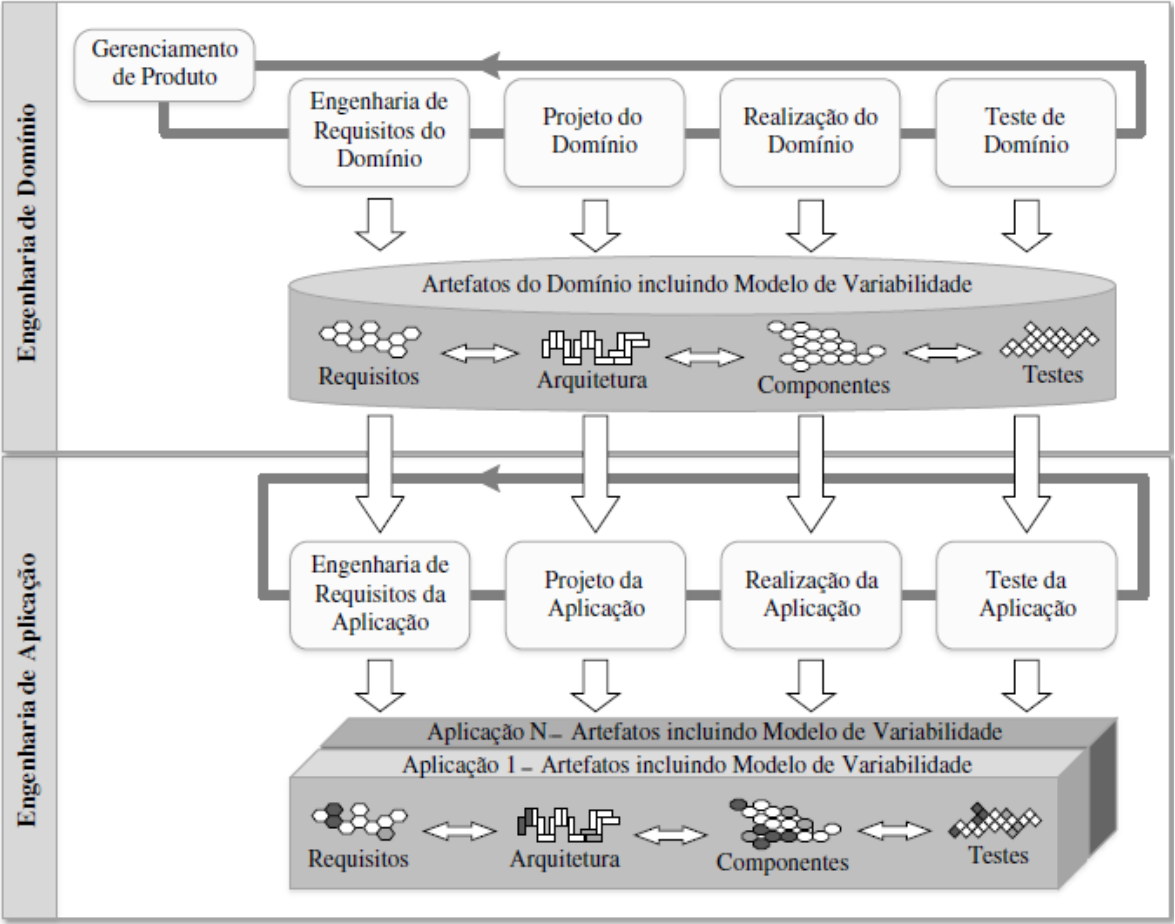
\includegraphics[scale=.37]{framewor_lps.png}}
	
	\caption{\textit{Framework} de Engenharia de LPS (Pohl et al., 2005). Traduzido por Geraldi (2015) }
	\label{fig:framework-lps}
\end{figure}


\section{Experimentos e \textit{Quasi}-Experimento em Engenharia de Software}
\label{sec:exp_eng_software}

Existe uma diferença relevante entre experimento e \textit{quasi}-experimento, esta diferença está relacionada a amostra do experimento. Quando se trata de um experimento a amostra é uma representação aleatória e válida de uma determinada população, ou seja, a amostra é uma representação da população. Quando se trata de \textit{quasi}-experimento a amostra não é aleatória e não representa sua população. É difícil realizar experimentos em LPS, devido a dificuldade de determinar uma amostra representativa e aleatória da população, pois normalmente estas amostras são pessoas \cite{wohlin2012experimentation}.

Por meio de um modelo teórico entre dois ou mais fenômenos relacionados a fim de determinar se este modelo proposto pode ser considerado correto, se desenvolve o experimento onde relacionamos a causa e o efeito deste modelo. Assim, utiliza-se o modelo para criar uma hipótese em relação às mudanças particulares nos fenômenos (a causa) que levarão a mudanças no outro (o efeito). Logo, o papel do experimento é testar a hipótese para decidir se é verdadeira ou falsa \cite{kitchenham2015evidence}. A \ref{fig:experimento} apresenta à ideia de uma relação causa e efeito em teoria, na qual a parte superior à linha trastejada se encontra a teoria e, na parte inferior a observação \cite{wohlin2012experimentation}.

\begin{figure}[htb]
	\centering					
	{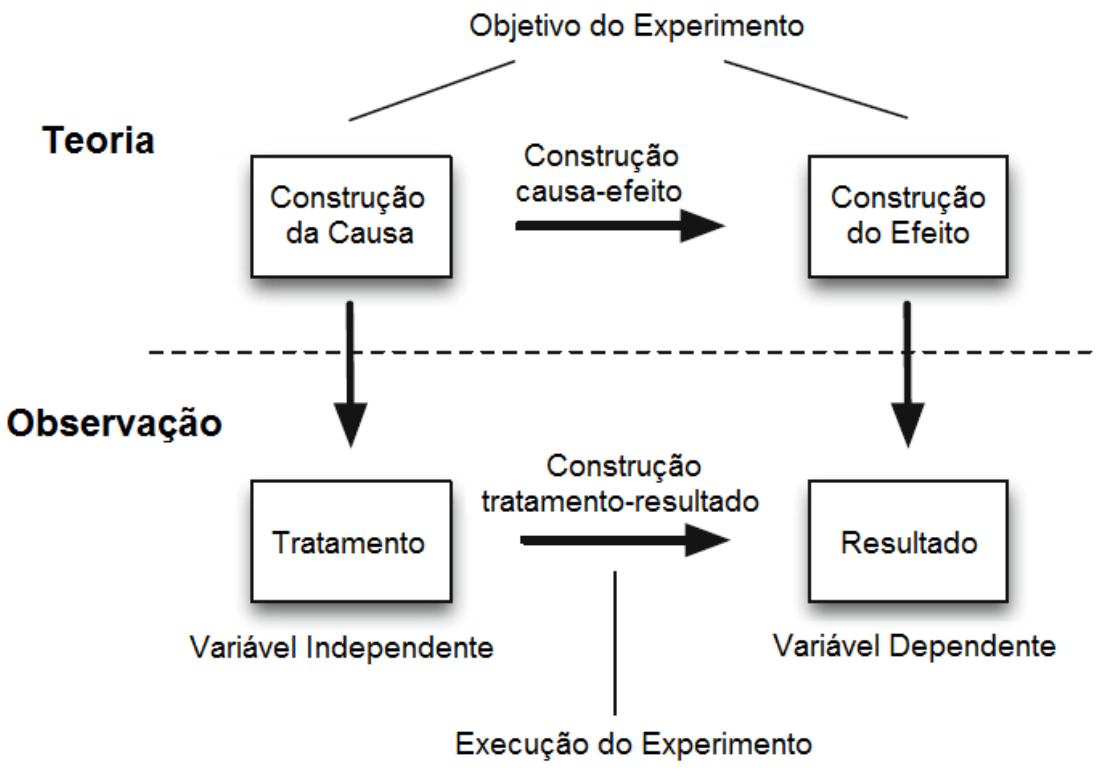
\includegraphics[scale=.37]{experimento.png}}
	
	\caption{Conceitos Essenciais de um Experimento. Traduzido de \citet{wohlin2012experimentation} }
	\label{fig:experimento}
\end{figure}

Um dos principais elementos de um experimento são as variáveis dependentes e independentes. 

\begin{itemize}
	\item \textbf{Variáveis independentes:} estão associadas à causa e controladas como resultado das atividades do experimentador, também são chamadas de fatores que podem assumir valores denominados tratamentos;
	\item \textbf{Variáveis dependentes:} estão associadas ao efeito e resultam nas mudanças que o experimentador realiza nas variáveis independentes \cite{kitchenham2015evidence}. 
\end{itemize}

Segundo \citealt{kitchenham2015evidence}, existe uma característica dita fator de confusão em experimentos de ES que envolvem seres humanos. Esse fator pode ser representado pela presença de algum elemento indesejável no estudo que dificulta distinguir entre duas ou mais causas possíveis de um efeito que foi medido pela variável dependente como, por exemplo, os níveis de habilidade dos participantes e a extensão de suas experiências anteriores com o objeto experimental.

Em Engenharia de Software, especialmente em LPS, é difícil de se executar experimentos dado que estes devem possuir aleatoriedade completa em suas variáveis. Isto se deve à dificuldade de alocar os participantes e/ou objetos a diferentes tratamentos de maneira aleatória, bem como, à falta de representatividade do número de participantes em uma amostra da população. Portanto, os experimentos realizados nesta área são, frequentemente, \textit{quasi}-experimentos, nos quais não há aleatoriedade dos participantes e/ou dos objetos experimentais, em ES chamados de artefatos de software, podendo ser processos ou ferramentas \cite{wohlin2012experimentation}.

Segundo \citealt{wohlin2012experimentation} a realização de um experimento pode ser dividido em um processo contendo cinco atividades, conforme apresentadas na \ref{fig:proc_exp} e descritas a seguir:

\begin{figure}[htb]
	\centering					
	{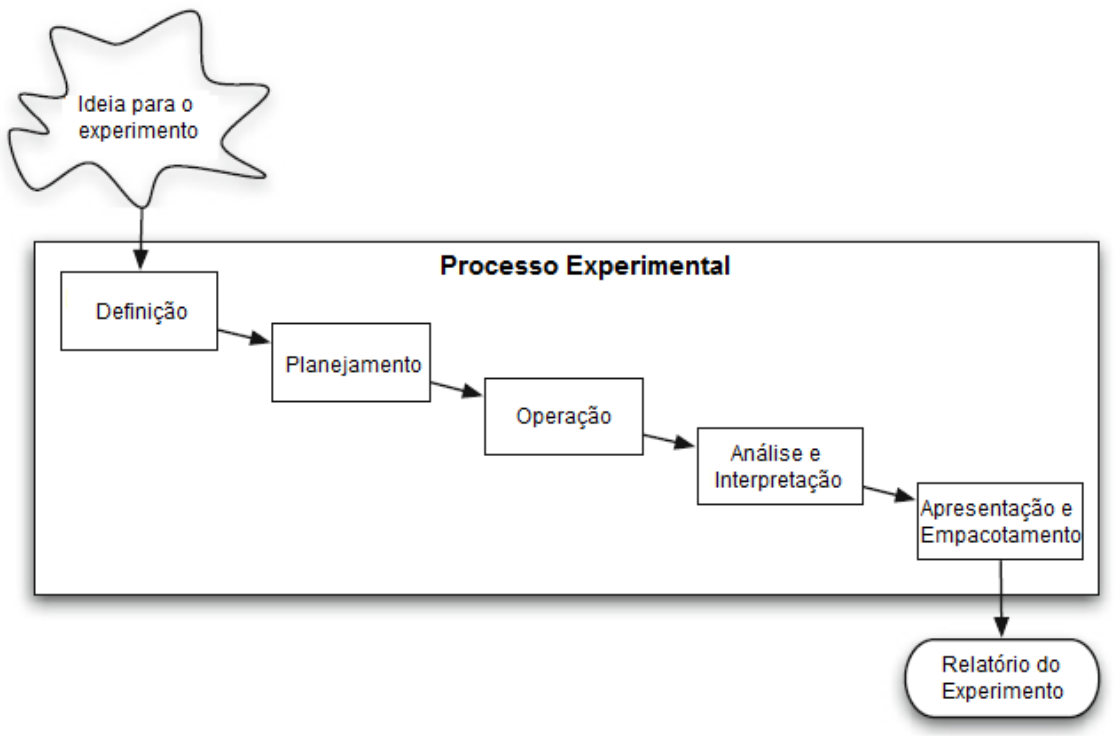
\includegraphics[scale=.37]{proc_exp.png}}
	
	\caption{Visão Geral do Processo Experimental. Traduzido de \citet{wohlin2012experimentation}}
	\label{fig:proc_exp}
\end{figure}


\begin{itemize}
	\item \textbf{Definição:} é a primeira atividade, onde define-se o problema, objetivo e metas do experimento. Caso não seja devidamente estabelecida, pode ocorrer retrabalho ou o experimento não pode ser utilizado para se estudar o que era almejado;

	\item \textbf{Planejamento:} é uma preparação de como o experimento será conduzido, em que ocorre a determinação do contexto do experimento, a formulação das hipóteses, sendo \textbf{hipótese nula} que o experimentador espera rejeitar com a maior confiança possível e a \textbf{hipótese alternativa} que se espera aceitar, a seleção de variáveis (dependentes e independentes), a seleção dos participantes, o projeto do experimento, a instrumentação e a avaliação da validade, dividida em quatro tipos, sendo \textbf{validade interna} refere-se ao relacionamento tratamento-resultado; \textbf{validade externa} apresenta a generalização dos resultados a uma população maior; \textbf{validade de \textit{constructo}} demonstra a relação entre a teoria e observação; e \textbf{validade de conclusão} refere-se a como os experimentadores foram aptos de analisar os resultados de um estudo e se a forma como foi feita é apropriada \cite{kitchenham2015evidence}.

	\item \textbf{Operação:} essa atividade é composta da \textbf{preparação} dos participantes e dos materiais necessários (instrumentação); \textbf{execução} das tarefas pelos participantes de acordo com diferentes tratamentos e coleta dos dados; e \textbf{validação dos dados} pelo experimentador, verificando os dados informados pelos participantes, de forma que os resultados do experimento sejam válidos; 
	
	\item \textbf{Análise e Interpretação:} os dados coletados na atividade anterior são analisados utilizando a estatística descritiva. Após isso, é verificada a necessidade de redução do conjunto de dados, de forma a garantir que os dados representam uma informação correta e/ou esperada. Por fim, realiza-se o teste de hipóteses para avaliar estatisticamente se hipótese nula pôde ser rejeitada. 
	
	\item \textbf{Apresentação e Empacotamento:} nessa atividade, os resultados são reportados, por exemplo, como artigos em conferência e/ou periódico, relatórios de tomada de decisão e empacotados para permitir a replicação do experimento, como material educativo, entre outros.
\end{itemize}

\section{Qualidade de Experimentos em Engenharia de Software}
\label{sec:qual_exp_eng_software}

Segundo \citet{dieste2013challenges}, o conceito de qualidade de experimentos em ES pode ser visto em dois pontos de vista diferentes, o primeiro é considerar a qualidade como o resultado da validade interna de um bom experimento e o segundo é tornar a qualidade operacional assim como a quantidade de vieses nos resultados experimentais. Outro ponto colocado por \citeauthor{dieste2013challenges}, é a validade externa que também tem uma função chave ao analisar se um experimento tem boa qualidade, porém essa função é contrária à validade interna.

Na \ref{tab:conceito_qualidade} são apresentadas as definições dos conceitos de qualidade citados anteriormente.

% Please add the following required packages to your document preamble:
% \usepackage{booktabs}
\begin{table}[]
	\centering
	\caption{Definições dos conceitos de qualidade em experimentos em Engenharia de
		Software. Traduzido de \citet{kitchenham2007large}}
	\label{tab:conceito_qualidade}
	\begin{tabular}{@{}lll@{}}
		\toprule
		Termo & Sinônimo & Definição \\ \midrule
		Viés & Erro sistemático & \begin{tabular}[c]{@{}l@{}}Uma tendência para produzir resultados \\ que partem sistematicamente de resultados \\ "verdadeiros". Resultados sem viés são\\ válidos internamente.\end{tabular} \\
		Validade Interna & Validade & \begin{tabular}[c]{@{}l@{}}O alcance em que o projeto e a condução \\ do estudo são possíveis de evitar erro sistemático. \\ A validade interna é um pré-requisito \\ para a validade externa.\end{tabular} \\
		Validade Externa & \begin{tabular}[c]{@{}l@{}}Generabilidade, \\ Aplicabilidade\end{tabular} & \begin{tabular}[c]{@{}l@{}}O alcance em que os efeitos observados no estudo \\ são aplicáveis fora do estudo.\end{tabular} \\ \bottomrule
	\end{tabular}
\end{table}

Segundo \citet{dieste2011systematic} os experimentos de boa qualidade são aqueles livres de vieses. O viés está relacionado com a validade interna, por exemplo, quão bem os experimentos são planejados, executados e analisados \cite{dieste2013challenges}. Para minimizar os vieses existem alguns métodos como, aleatorização para criar grupos experimentais homogêneos, imparcialidade para alocar os indivíduos. Desta forma os resultados podem ser analisados mesmo depois do experimento ter sido realizado com replicações. Enquanto os experimentos de baixa qualidade seriam os que usam pouco ou nenhum dos métodos citados \cite{dieste2011systematic}.

Como o viés não pode ser medido, existem algumas abordagens para avaliá-lo. Os instrumentos de Avaliação de Qualidade (AQ), são projetados para avaliar a validade interna e inferir a qualidade de experimentos, tais como, abordagens simples (questionários), \textit{checklists} (contem ou não contem), escalas de qualidade, opinião de especialista \cite{dieste2011systematic,dieste2013challenges,teixeira2014analise}.

Por outro lado a qualidade de um experimento em ES também pode ser avaliada considerando o projeto e análise dos experimentos, em termos de poder estatístico, análise do tamanho de efeito (resultado), \textit{quasi}-experimentais e relatório de experimento \cite{kampenes2007quality}.

Até o momento não se tem conhecimento de trabalhos que tratam a qualidade de experimentos em área especifica de ES. Entretanto, foram recuperados alguns trabalhos, por meio de pesquisas não sistemáticas, que estão relacionados com a avaliação de qualidade dos experimentos em Engenharia de Software, descritos a seguir:

\begin{itemize}
	\item \citet{kitchenham2007large} propõem um \textit{checklist} de avaliação de qualidade de experimentos em ES contendo cinquenta questões para avaliar a qualidade de experimentos, em que sugerem que os pesquisadores selecionem apenas as questões do \textit{checklist} mais adequadas ao contexto de suas próprias questões de pesquisa.
	
	\item \citet{kitchenham2015evidence} apresentam um \textit{checklist} de avaliação de qualidade de experimentos em ES com nove questões, onde cada questão possui subquestões	categorizadas em: (i) "Questões sobre objetivo", (ii) "Questões sobre o projeto, coleta de dados e análise do dados" e (iii) "Questões sobre o resultado do estudo".
	
	\item \citet{dieste2011systematic}  desenvolveram uma escala de qualidade para determinar a qualidade de experimentos, contendo dez questões baseadas nas cinco dimensões de \citet{kitchenham2007large}, sendo: contexto experimental, projeto experimental, análise, interpretação dos resultados e apresentação dos resultados. As respostas de cada questão são "sim" ou "não".	
\end{itemize}


\section{Ontologia}
\label{sec:ontologia}

A palavra ontologia é formada por meio dos termos gregos ontos (ser) e logos (estudo, discurso), que engloba algumas questões abstratas como a existência de determinadas entidades, o que se pode dizer que existe, qual o significado do ser, etc. Segundo \citet{wolff1962philosophia}, ontologia é um ramo da filosofia que estuda a realidade e existência, ou o ser enquanto ser. Em outras palavras, é o estudo da descrição de coisas do mundo real. Outro ponto de vista proposto por \citet{gruber1993ontology}, diz que ontologias são uma especificação formal de uma contextualização e uma contextualização é uma visão abstrata e simplificada do mundo.

Ontologia em Computação, Sistemas de Informação e Ciência da Informação, é definida como um modelo de dados que representa um conjunto de conceitos dentro de um domínio e os relacionamentos entre estes. Uma ontologia é utilizada para realizar inferência sobre os objetos do domínio. No cenário atual, as ontologia em ciências da informação são utilizadas como uma forma de representação de conhecimento lógico, possibilitando a inferência de novos fatos com base nos dados armazenados na ontologia.

Uma ontologia define primitivas/diretrizes de um domínio de conhecimento, estas primitivas/diretrizes podem ser definidas como classes, atributos, propriedades e restrições. Essas definições seguem o padrão de representação conhecido como lógica descritiva. A lógica descritiva representa os conceitos de um domínio (chamado de \textbf{TBox} - \textit{Terminological Box}) separadamente dos indivíduos (chamado de \textbf{ABox} - \textit{Assertion Box}) \cite{calvanese2005dl}. A lógica descritiva é mais representativa e eficiente que a lógica proposicional e a lógica de predicados (usados em linguagens de programação lógica, como Prolog).

Portanto uma ontologia para a representação de um conhecimento possui a seguinte estrutura: Uma base de conhecimento onde estão os dois conjuntos de conhecimento terminológico (\textbf{TBox}) e o conjunto de conhecimento sobre objetos (\textbf{ABox}), seguido de um mecanismo de inferência e uma aplicação para atuar na manipulação de informações extraídas do mecanismo de inferência, A \ref{fig:estrct_onto} apresenta essa estrutura.

\begin{figure}[htb]
	\centering					
	{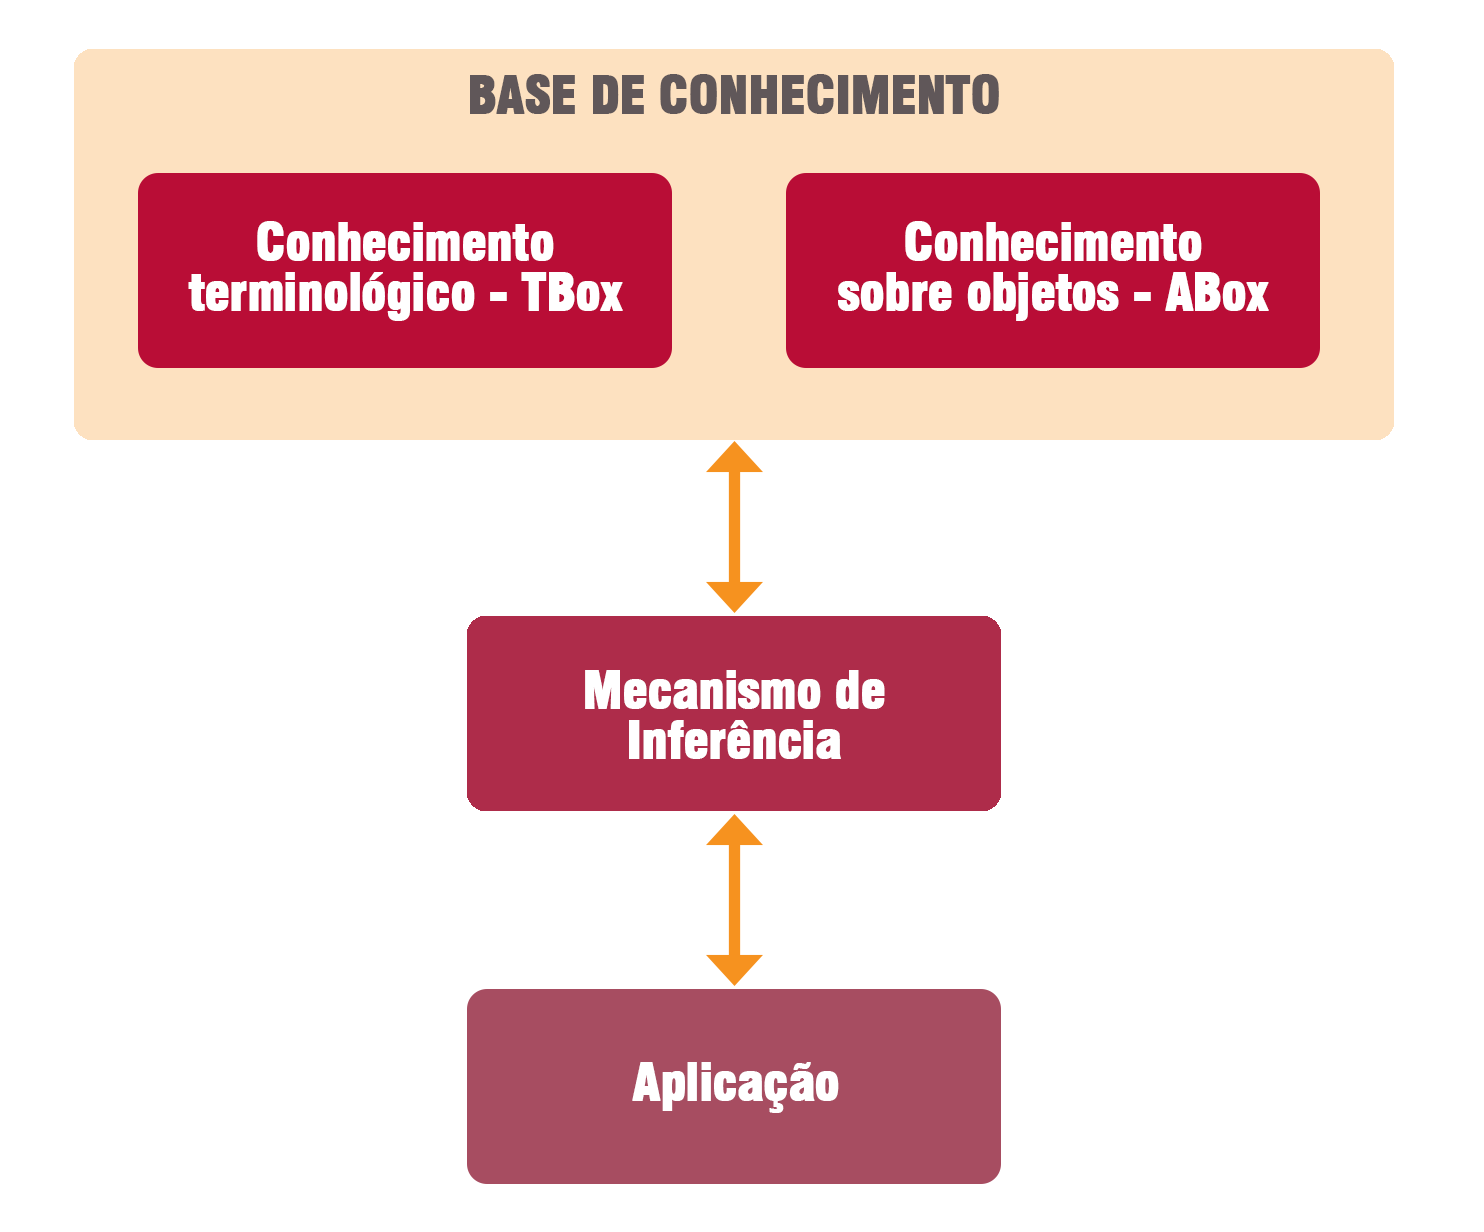
\includegraphics[scale=.7]{estrutura_ontologia.png}}
	
	\caption{Estrutura de uma Ontologia. Autor}
	\label{fig:estrct_onto}
\end{figure}

\begin{figure}[htb]
	\centering					
	{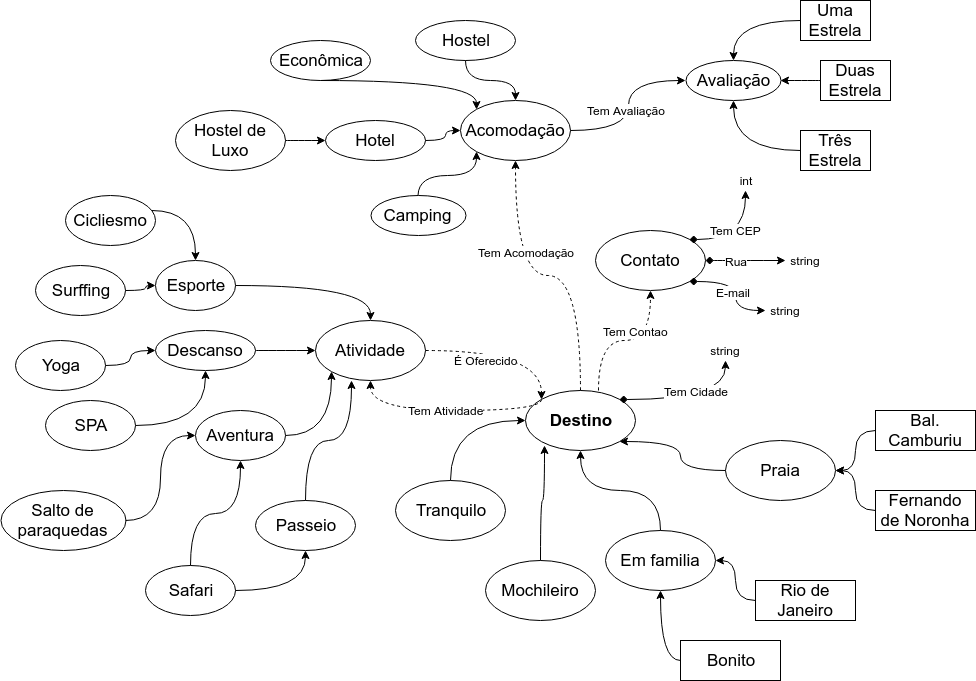
\includegraphics[scale=0.45]{exemplo_ontologia.png}}
	
	\caption{Exemplo de uma Ontologia para o domínio: Destino de Viagem. Autor}
	\label{fig:exemplo_ont}
\end{figure}

A \ref{fig:exemplo_ont} apresenta um exemplo de ontologia, por meio de um grafo, para o domínio: "destino de viagem". Os vértices ovais representam as classes, e os vértices retangulares representam os indivíduos (instâncias da classe). As arestas comuns representa um relacionamento de classe e subclasse, as arestas trastejadas representam um relacionamento de propriedade, já as arestas que começam com um losango indica a definição de uma propriedade, especificando sua tipagem.


\section{Sistema de Recomendação}
\label{sec:sit_recmendacao}

Os sistemas de recomendação são aplicativos de software que visam dar suporte para usuário na tomada de decisões ao interagir com grandes espaços de informação. Estes softwares recomendam itens de interesse para os usuários com base em preferências que tenham sido expressas explicitamente ou implicitamente \cite{ricci2011introduction}. Segundo \citet{mahmood2009improving} os sistemas de recomendação são técnicas ou ferramentas de software, que podem reduzir a sobrecarga de informações para os usuários, sugerindo itens, conteúdos ou serviços, entre outros.

\subsection{Sistemas de Recomendação Tradicional}

Os sistemas de recomendação surgiram nos trabalhos extensivos das ciências cognitivas, teoria de aproximação, recuperação da informação e teoria de previsões e também possuem influências das ciências de administração e marketing \cite{allen2001econometric, murthi2003role}. O primeiro sistema de recomendação proposto foi o \textit{Tapestry}, nesse sistema criou-se um modelo mais usados em sistemas de recomendação, onde a recomendação de conteúdo é auxiliada pela colaboração de um grupo de pessoas, batizada como "filtragem  colaborativa". Nesse trabalho, iniciou o desafio de casar corretamente os que dados recomendados com os usuários que o recebem, analisando o real relacionamento de interesse \cite{kwong1992dynamic, resnick1997recommender}.

Podemos apresentar uma definição formal para sistema de recomendação da seguinte forma: 

\newtheorem{mydef}{Definicão}
\begin{mydef}
	Seja $C$ o conjunto de todos os usuários de um determinado sistema, e seja $S'$ o conjunto de todos os possíveis itens que podem ser recomendados como livros, filmes, restaurantes etc. Seja $u$ a função utilidade que mede o quão útil é um determinado item s para um determinado usuário $c$, \textbf{\textit{u}:C x S $\rightarrow$ R}, onde $R$ é um conjunto totalmente ordenado segundo a função utilidade. Então, para cada usuário \textbf{\textit{c} $\in$ C}, procura-se um item \textbf{\textit{s'} $\in$ S} que maximiza a utilidade do usuário. Isto pode ser expressado pela equação \ref{eq:form_sis_rec}:
	
	\begin{equation}
	\label{eq:form_sis_rec}
	\forall c \in C, s'_{c} = argmax_{s \in S u(c, s)}
	\end{equation}
	
	Em um sistema de recomendação a utilidade de um item é geralmente representada por uma avaliação que indica o quanto um determinado usuário gosta de um item. No entanto, conforme descrito na definição acima, a função de utilidade pode ser uma função arbitrária.
	
	Cada elemento dos usuários $C$ pode ser definido por um perfil que inclui as características do usuário, por exemplo, a sua idade, sexo, etc. No caso mais simples, o perfil pode conter um único elemento como um identificador único (ID). Da mesma forma, cada item de $S$ pode ser definido por um conjunto de características. Por exemplo, na recomendação de filmes, na qual $S$ é a coleção de filmes, cada filme pode ser representado não apenas pelo seu ID, mas também pelo seu título, gênero, diretor, ano de lançamento, etc.
\end{mydef}

Exitem cinco abordagens mais usadas em sistemas de recomendação, três tradicionais: Filtragem Colaborativa (\textit{Collaborative Filtering}), Filtragem Baseada em Conteúdo (\textit{Content-based Filtering}) e Recomendação Baseada no Conhecimento (\textit{Knowledge-Based Recommendation}), e duas modernas: Sistemas de Recomendação Híbridos \textit{(Hybrid Recommender Systems}) e Sistemas de Recomendação usando Informações de Contexto (\textit{Context-aware Recommender Systems}).

\begin{itemize}
	\item \textbf{\textit{Collaborative Filtering}:}
	A Filtragem Colaborativa baseia-se na ideia de "boca-a-boca" em que a informação passada de pessoa a pessoa desempenha um papel importante ao tomar uma decisão. Abstraindo, as pessoas são substituídas pelos chamados vizinhos mais próximos (NN) que são usuários com um padrão de preferência ou comportamento semelhante ao usuário atual. \cite{robillard2010recommendation}. Filtragem Colaborativa depende de dois tipos diferentes de dados: (1) um conjunto de usuários e (2) um conjunto de itens. A relação entre usuários e itens é expressada principalmente em termos de \textit{ratings} fornecidos pelos usuários e explorados em futuras sessões de recomendação para prever a classificação de um usuário \cite{robillard2010recommendation}.
	
	\item \textbf{\textit{Content-based Filtering}:}
	A Filtragem Baseada em Conteúdo tem como característica principal o pressuposto de interesses pessoais, por exemplo, os usuários interessados no tópico de qualidade de experimentos em LPS normalmente não alteram seu interesse de um dia para outro, mas também estarão interessados em um tópico próximo, como por exemplo experimentos em Sistema de Sistemas. Abstraindo, as abordagens de recomendação baseadas em conteúdo são aplicadas, por exemplo, quando se trata da recomendação de sites (notícias com conteúdo semelhante em comparação com o conjunto de notícias já consumidas) \cite{robillard2010recommendation}. Filtragem Baseada em Conteúdo depende de dois tipos diferentes de dados: (i) um conjunto de usuários e (ii) um conjunto de categorias (ou palavras-chave) atribuídas ou extraídas dos itens (descrições de itens). Os sistemas de recomendação de filtragem baseados em conteúdo calculam um conjunto de itens que são mais parecidos com itens já conhecidos pelo usuário atual \cite{robillard2010recommendation}.

	\item \textbf{\textit{Knowledge-Based Recommendation}:} 
	A recomendação baseada no conhecimento, baseia-se nos seguintes	dados básicos: (i) um conjunto de regras (restrições) ou métricas de similaridade e (ii) um conjunto de itens. Dependendo dos requisitos do usuário, regras (restrições) que descrevam quais itens devem ser recomendados. O usuário atual articula suas necessidades (preferências) em termos de especificações e propriedades de itens que são internamente bem representados em termos de regras (restrições).
	
	\item \textbf{\textit{Hybrid Recommender Systemson}:}
	São algoritmos que combinam \textit{Collaborative Filtering} com \textit{Content-based Filtering} e podem ser feitos de diversas formas diferentes, por exemplo, aplicando os dois separados e juntando os resultados depois, adicionando a saída de um ao outro ou unificando as duas abordagens em um único modelo. Alguns exemplos são as abordagens baseada em pesos, misturadas a cascatas \cite{jannach2010recommender}.
	
	
	\item \textbf{\textit{Context-aware Recommender Systems}:} 
	Existem casos de recomendações que não podem levar em consideração somente os dados do item ou do usuário, como conteúdo personalizado de um site de filmes, sites de viagens e até sites de notícias. A incorporação do contexto permite personalizar ainda mais a recomendação e criar experiências realmente válidas ao usuário. Segundo \citet{rahman2013ide} \textit{Context-aware Recommender Systems}, segue as abordagens anteriores assumindo a existência de certos fatores contextuais como, por exemplo, o tempo e a localização, que identificam o contexto no qual as recomendações são fornecidas. Eles assumem que cada um desses fatores contextuais podem ter uma estrutura. O fator Tempo, por exemplo, pode ser definido em termos de segundos, minutos, horas, dias, meses e anos. \citet{rahman2013ide} cita como classificar o contexto baseando-se nos seguintes aspectos, (i) o que um sistema de recomendação pode saber sobre esses fatores contextuais e (ii) como os fatores contextuais mudam ao longo do tempo. Desta forma podemos definir este tipo de sistema de recomendação pela formula \ref{eq:form_sis_rec_ca}
	
	\begin{equation}
		\label{eq:form_sis_rec_ca}
		f:User \times Item \times Context \rightarrow Rating
	\end{equation}

\end{itemize}


\subsection{Sistema de Recomendação em Engenharia de Software}

Em Engenharia de Software (\textit{Recommendation System in Software Engineering} - RSSEs), sistemas de recomendação desempenham importantes funções a fim de ajudar a equipe de software a lidar com sobrecarga de informações, filtrando e fornecendo informações úteis. São ferramentas de software introduzidas especificamente para ajudar equipes de desenvolvimento de software e partes interessadas a lidar com a busca de informações em um determinado contexto em ES \cite{robillard2010recommendation}.

\citet{robillard2010recommendation} comenta que, em um ambiente de desenvolvimento de software aplicando ES existe um \textit{landscape} de informações sobre o projeto em desenvolvimento, e este espaço de informações pode ser categorizados por:

\begin{itemize}
	\item Código fonte do projeto;
	\item História do projeto;
	\item Arquivos de comunicação;
	\item Dependências de API em outras fontes;
	\item Ambiente de desenvolvimento;
	\item Logs de interação entre os usuários;
	\item Logs de execução e;
	\item A web.
\end{itemize}

Um RSSE pode trazer simultaneamente dois aspectos distintos: (i) novidade e surpresa, porque as RSSEs ajudam a descobrir novas informações e (ii) traz familiaridade e reforço, pois as RSSEs suportam a confirmação do conhecimento existente. Finalmente, referenciar uma tarefa e um contexto específicos, distingue RSSEs de ferramentas de pesquisa genéricas, por exemplo, uma ferramentas de RSSR para ajudar os desenvolvedores a encontrar exemplos de código fonte \cite{robillard2010recommendation}.

RSSE compreende três componentes principais, (i) um mecanismo para coletar dados, (ii) um mecanismo de recomendação para analisar dados e gerar recomendações e (iii) uma interface de usuário para fornecer recomendações \cite{rahman2014towards}.

\begin{figure}[htb]
	\centering					
	{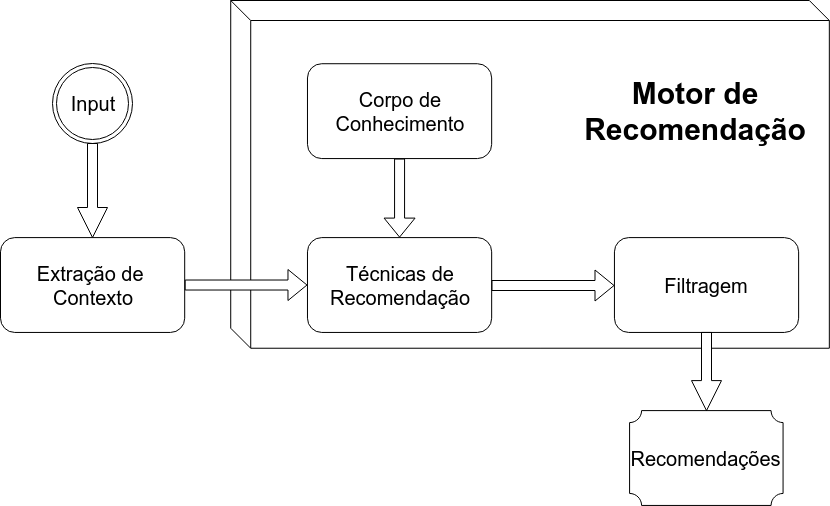
\includegraphics[scale=.5]{rsse.png}}
	
	\caption{Passos de Construção para um RSSE. Traduzido e Adaptado de \citet{maki2016systematic}}
	\label{fig:rsse}
\end{figure}

A \ref{fig:rsse} apresenta de forma geral como é construído um RSSE, partindo da entradas dos dados pelo \textit{input}, passando pela extração de contexto, seguindo para aplicação de alguma técnica de recomendação, na qual sofre um inferência do corpo de conhecimento (normalmente especifico para cada área de ES), depois segue pra um processo de filtragem dos resultados, e como saída a recomendação em si.

Foi encontrado uma revisão sistemáticas (trabalho da \citealp{maki2016systematic}), que aborda métodos e modelos de implementação de um RSSE apresentando vários aspectos de SR em ES, principalmente no tipo de corpo de conhecimento aplicado a RSSE. Nessa revisão foi possível identificar algumas áreas da ES que utiliza SR, apresentadas a seguir.

\begin{itemize}
	\item SR para exploração código fonte;
	\item SR para reuso de software;
	\item SR para refatoração de código fonte (por exemplo, \textit{class} em POO);
	\item SR para reuso de componentes de software;
	\item SR na exploração de APIs;
	\item SR na depuração de código (\textit{debugging})
	\item SR na recomendação de agentes \textit{Agile}
	\item SR na descoberta de requisitos;
	\item SR na mudança do ciclo de vida;
	\item SR na evolução do ciclo de vida e;
	\item SR na busca de \textit{bugs}.
\end{itemize}

Por meio deste estudo, foi possível identificar em qual domínio de aplicação da industria de ES estão aplicando qual técnica de SR, apresentados na \ref{tab:tec_x_doman} a seguir.

\begin{table}[]
	\centering
	\caption{Sumário de técnicas de recomendação em cada domínio, Traduzido e Adaptado de \citet{maki2016systematic} }
	\label{tab:tec_x_doman}
	\begin{tabular}{@{}llllllllll@{}}
		\toprule
		\multicolumn{1}{c}{\textbf{Domínios}} & \multicolumn{8}{c}{\textbf{Técnicas}} & \multicolumn{1}{c}{\textbf{\begin{tabular}[c]{@{}c@{}}Número de \\ Referências\end{tabular}}} \\ \midrule
		& CBF & CF & KBF & Hibrido & IA & \begin{tabular}[c]{@{}l@{}}Redes \\ Sociais\end{tabular} & \begin{tabular}[c]{@{}l@{}}Info. de\\ Contexto\end{tabular} & \begin{tabular}[c]{@{}l@{}}Grupo de \\ agregação\end{tabular} &  \\ \midrule
		Governo & 1 & 5 & 1 & 5 & 4 &  &  &  & 9 \\
		Negócios &  & 1 & 3 & 3 & 4 &  &  &  & 5 \\
		Comercio & 3 & 1 & 4 & 1 & 4 & 2 &  &  & 8 \\
		Livraria & 2 & 2 &  & 3 & 1 &  &  &  & 6 \\
		Escolas & 2 &  & 11 &  & 1 &  &  &  & 10 \\
		Turismo & 5 & 9 & 9 & 9 & 2 & 2 & 11 &  & 18 \\
		Pesquisa & 9 & 16 & 6 & 15 & 3 & 1 & 1 &  & 27 \\
		\begin{tabular}[c]{@{}l@{}}Grupo de \\ Atividade\end{tabular} & 9 & 5 & 2 & 5 & 8 &  &  & 2 & 21 \\
		\textbf{Total} & \textbf{31} & \textbf{39} & \textbf{36} & \textbf{41} & \textbf{27} & \textbf{5} & \textbf{12} & \textbf{2} & \textbf{104} \\ \bottomrule
	\end{tabular}
\end{table}

\section{Trabalhos Relacionados}

Até o momento não há trabalhos de sistema de recomendações para recomendar experimentos em ES, nem em LPS. Outros trabalhos relacionados mais próximos já foram apresentado na Seção 2.3 e não são objetos de evolução de experimento gerais em ES.

Encontramos alguns estudos que propuseram abordagens para representar formalmente dados sobre experimentos de SE.

A revisão da literatura mostrou que a maioria dos estudos focalizou a representação de todo o domínio do SE. Isso é muito complexo devido à quantidade de detalhes de cada campo. Em vez disso, nos concentramos primeiro em um campo de SE devido à nossa experiência em grupo.

Durante nossa revisão de literatura encontramos: \cite{garcia2008ontology} Ontologia para Experimentos Controlados em Engenharia de Software, \cite{scatalon2011packaging} Empacotando Experimentos Controlados Usando uma Abordagem Evolutiva Baseada em Ontologia (S), \cite{da2012foundational} Uma Ontologia Fundamental para Apoiar Experimentos Científicos, \cite{blondet2016ode} ODE: uma Ontologia para Projeto Numérico de Experimentos, \cite{soldatova2006ontology} Uma Ontologia de Experimentos Científicos, \cite{gelernter2016challenges} Desafios na Avaliação de Ontologia, \cite{cruzes2007extracting} Extraindo Informações da Engenharia de Software Experimental papéis. No entanto, todos esses trabalhos não tratam experimentos de SPL.

O trabalho de Garcia et al. \cite{garcia2008ontology}, Poveda-Villalón et al. \cite{scatalon2011packaging} e Cruz et al. \cite{da2012foundational} se destaca em nosso contexto por propor e modelar ontologias específicas para experimentos em engenharia de software. O trabalho de \cite{garcia2008ontology} propõe, através de diagramas de classes UML, uma ontologia para experimentos controlados em engenharia de software denominada EXPEROntology. Com o objetivo de ser uma ferramenta de transferência de conhecimento para auxiliares de pesquisadores e revisores, além de propor meta-análises, conduzir e avaliar experimentos controlados. O trabalho de Poveda-Villalón et al. \cite{scatalon2011packaging} é uma evolução do trabalho de Garcia et al. \cite{garcia2008ontology}, mas focado na evolução desta ontologia proposta. O trabalho de Cruz et al. \cite{da2012foundational} apresenta uma ontologia chamada OVO (Open onVence Ontology) na qual é inspirada por três teorias: (i) O ciclo de vida de experimentos científicos, (ii) Open Provent (OPM) e (iii) Unified Foundational Ontology ( OVNI) Este modelo OVO pretende ser uma referência para modelos conceituais que podem ser usados ??por pesquisadores para explorar a semântica de metadados.

Por outro lado, os trabalhos de Blondet et al. \cite{blondet2016ode} e Soldatova e King \cite{soldatova2006ontology} tratam ontologias no contexto geral de experimentos. O trabalho de Blondet et al. \cite{blondet2016ode} traz uma proposta de ontologia para DoE (Designs of Experiments) para apoiar as decisões de processo sobre o DoE. O trabalho de Soldatova e King \cite{soldatova2006ontology} propõe a ontologia da EXPO que é uma mediana da ontologia SUMO (Suggested Upper Merged Ontology). Esta ontologia visa especificar os experimentos formalizando e generalizando os conceitos de design, metodologias e representação de resultados. Este trabalho é o único que usa o modelo OWL-DL para representar a ontologia.

O trabalho de Gelernter e Jha \cite{gelernter2016challenges} dá uma visão geral sobre os desafios de avaliar uma ontologia, mas não trata da ontologia para experimentos.

Finalmente, o trabalho de Cruzes et al. \cite{cruzes2007extracting} trata de uma técnica para extrair meta-informação de experimentos em engenharia de software, entendemos que este assunto está relacionado a este artigo, pois estaremos gerando através da ontologia proposta diversos metadados sobre experimentos em SPL.

A revisão da literatura mostrou que a maioria dos estudos focalizou a representação de todo o domínio do SE. Isso é muito complexo devido à quantidade de detalhes de cada campo. Em vez disso, nos concentramos primeiro em um campo de SE devido à nossa experiência em grupo.